\documentclass[11pt]{beamer}
\usetheme[nat,greyfoot,footstyle=low,headstyle=institute,style=alternative]{Frederiksberg}

\usepackage[utf8]{inputenc}
\usepackage[english]{babel}
\usepackage{times}

\usepackage{amsmath}
\usepackage{amssymb}

\usepackage{xcolor}
\usepackage{color}
\usepackage[outputdir=.tmp,cache=false]{minted}
% \setminted{frame=lines,linenos,framesep=2mm,fontsize=\small}

\usepackage{url}
\def\CC{{C\nolinebreak[4]\hspace{-.05em}\raisebox{.4ex}{\tiny ++}}}

\usepackage{pgfplots}
\usepgfplotslibrary{units}
\pgfplotsset{compat=newest}

\pgfplotsset{
  every axis plot post/.style={/pgf/number format/fixed}
}
\usepackage{graphicx}
\usepackage[caption=false,font=footnotesize]{subfig}
\newsubfloat{figure}

\usepackage{cspsymb}

\normalfont
%\usepackage[T1]{fontenc}
% \renewcommand{\ttdefault}{cmtt}
\usepackage{booktabs, caption, siunitx}

\usepackage{tikz}


\usepackage[labelsep=period]{caption}

\usetikzlibrary{calc}
\usetikzlibrary{fit}
\usetikzlibrary{positioning}
\usepgfplotslibrary{units}
\pgfplotsset{compat=newest}

\usetikzlibrary{decorations.markings}
\usetikzlibrary{arrows}
\usetikzlibrary{shapes.geometric}

\usepackage{ifthen}
\pgfkeys{
  /sevenseg/.is family, /sevenseg,
  slant/.estore in      = \sevensegSlant,     % vertical slant in degrees
  size/.estore in       = \sevensegSize,      % length of a segment
  shrink/.estore in     = \sevensegShrink,    % avoids overlapping of segments
  line width/.estore in = \sevensegLinewidth, % thickness of the segments
  line cap/.estore in   = \sevensegLinecap,   % end cap style rect, round, butt
  oncolor/.estore in    = \sevensegOncolor,   % color of an ON segment
  offcolor/.estore in   = \sevensegOffcolor,  % color of an OFF segment
}

\pgfkeys{
  /sevenseg,
  default/.style={
    slant = 0,
    size = 1em,
    shrink = 0.2,
    line width = 0.3em,
    line cap = butt,
    oncolor = green,
    offcolor = black!75!green
  }
}
\newcommand{\sevenseg}[2][]% options values
{%
\pgfkeys{/sevenseg, default, #1}%
\def\sevensegarray{#2}%
  \begin{tikzpicture}%
    % first define the position of the 6 corner points
    \path (0,0) ++(0,0)                             coordinate (P1);
    \path (0,0) ++(\sevensegSize,0)                 coordinate (P2);
    \path (0,0) ++(90-\sevensegSlant:\sevensegSize) coordinate (P3);
    \path (P2)  ++(90-\sevensegSlant:\sevensegSize) coordinate (P4);
    \path (P3)  ++(90-\sevensegSlant:\sevensegSize) coordinate (P5);
    \path (P4)  ++(90-\sevensegSlant:\sevensegSize) coordinate (P6);
    % then step through the 1/0 values in the segment array
    \foreach \i in {0,...,6}%
    {
      \pgfmathparse{\sevensegarray[\i]}
      \ifthenelse{\equal{\pgfmathresult}{1}}%
        {\let\mycolor=\sevensegOncolor}%  segment is on
        {\let\mycolor=\sevensegOffcolor}% segment is off
      \tikzstyle{segstyle} = [draw=\mycolor, line width = \sevensegLinewidth,
                              line cap = \sevensegLinecap]
      %-----------------------
      \ifthenelse{\equal{\i}{0}}{\path[segstyle]
        (${1-\sevensegShrink}*(P5)+\sevensegShrink*(P6)$)
        -- ($\sevensegShrink*(P5)+{1-\sevensegShrink}*(P6)$);}{} % a
      \ifthenelse{\equal{\i}{1}}{\path[segstyle]
        (${1-\sevensegShrink}*(P6)+\sevensegShrink*(P4)$)
        -- ($\sevensegShrink*(P6)+{1-\sevensegShrink}*(P4)$);}{} % b
      \ifthenelse{\equal{\i}{2}}{\path[segstyle]
        (${1-\sevensegShrink}*(P4)+\sevensegShrink*(P2)$)
        -- ($\sevensegShrink*(P4)+{1-\sevensegShrink}*(P2)$);}{} % c
      \ifthenelse{\equal{\i}{3}}{\path[segstyle]
        (${1-\sevensegShrink}*(P1)+\sevensegShrink*(P2)$)
        -- ($\sevensegShrink*(P1)+{1-\sevensegShrink}*(P2)$);}{} % d
      \ifthenelse{\equal{\i}{4}}{\path[segstyle]
        (${1-\sevensegShrink}*(P1)+\sevensegShrink*(P3)$)
        -- ($\sevensegShrink*(P1)+{1-\sevensegShrink}*(P3)$);}{} % e
      \ifthenelse{\equal{\i}{5}}{\path[segstyle]
        (${1-\sevensegShrink}*(P3)+\sevensegShrink*(P5)$)
        -- ($\sevensegShrink*(P3)+{1-\sevensegShrink}*(P5)$);}{} % f
      \ifthenelse{\equal{\i}{6}}{\path[segstyle]
        (${1-\sevensegShrink}*(P3)+\sevensegShrink*(P4)$)
        -- ($\sevensegShrink*(P3)+{1-\sevensegShrink}*(P4)$);}{} % g
    }
  \end{tikzpicture}%
}

\newcommand{\sevensegnum}[2][]% sample characvters
{%
  \ifthenelse{\equal{#2}{0}}{\sevenseg[#1]{{1,1,1,1,1,1,0,}}}{%
  \ifthenelse{\equal{#2}{1}}{\sevenseg[#1]{{0,1,1,0,0,0,0,}}}{%
  \ifthenelse{\equal{#2}{2}}{\sevenseg[#1]{{1,1,0,1,1,0,1,}}}{%
  \ifthenelse{\equal{#2}{3}}{\sevenseg[#1]{{1,1,1,1,0,0,1,}}}{%
  \ifthenelse{\equal{#2}{4}}{\sevenseg[#1]{{0,1,1,0,0,1,1,}}}{%
  \ifthenelse{\equal{#2}{5}}{\sevenseg[#1]{{1,0,1,1,0,1,1,}}}{%
  \ifthenelse{\equal{#2}{6}}{\sevenseg[#1]{{1,0,1,1,1,1,1,}}}{%
  \ifthenelse{\equal{#2}{7}}{\sevenseg[#1]{{1,1,1,0,0,0,0,}}}{%
  \ifthenelse{\equal{#2}{8}}{\sevenseg[#1]{{1,1,1,1,1,1,1,}}}{%
  \ifthenelse{\equal{#2}{9}}{\sevenseg[#1]{{1,1,1,1,0,1,1,}}}{%
  \ifthenelse{\equal{#2}{A}}{\sevenseg[#1]{{1,1,1,0,1,1,1,}}}{%
  \ifthenelse{\equal{#2}{B}}{\sevenseg[#1]{{0,0,1,1,1,1,1,}}}{%
  \ifthenelse{\equal{#2}{C}}{\sevenseg[#1]{{0,0,0,1,1,0,1,}}}{%
  \ifthenelse{\equal{#2}{D}}{\sevenseg[#1]{{0,1,1,1,1,0,1,}}}{%
  \ifthenelse{\equal{#2}{E}}{\sevenseg[#1]{{1,0,0,1,1,1,1,}}}{%
  \ifthenelse{\equal{#2}{F}}{\sevenseg[#1]{{1,0,0,0,1,1,1,}}}{%
  {\sevenseg[#1]{{0,0,0,0,0,0,0,}}}}}}}}}}}}}}}}}}}%
}

\tikzset{
  myarrow/.style={
    draw=black,
    thick,
    ->,
    shorten <=3pt,
    shorten >=3pt,
  },
  mycircle/.style={
    draw=black,
    shape=circle,
    very thick,
    inner sep=3pt,
    inner ysep=5pt,
    text width=0.75cm,
    align=center,
    minimum size=0.75cm,
    rounded corners,
  },
  mytriangle/.style={
    draw=black,
    regular polygon,
    regular polygon sides=3,
    align=center,
    rounded corners,
    very thick,
    inner sep=3pt,
  },
  myrectangle/.style={
    draw=black,
    shape=rectangle,
    very thick,
    rounded corners,
    align=center,
    inner sep=7pt,
    inner ysep=7pt,
    text width=2.1cm,
    minimum size=0.5cm,
    minimum height=1.5cm,
    font=\footnotesize
  },
  mysquare/.style={
    draw=black,
    shape=rectangle,
    very thick,
    rounded corners,
    align=center,
    inner sep=7pt,
    inner ysep=7pt,
    font=\footnotesize
  }
}

\pgfplotsset{
  every axis plot post/.style={/pgf/number format/fixed}
}

% \newsavebox{\smeilexamplecode}
% \begin{lrbox}{\smeilexamplecode}
%   \begin{minipage}{1.1\textwidth}
%     \begin{minted}[fontsize=\scriptsize, frame=none, linenos, framesep=2mm, autogobble, escapeinside=||, mathescape=true]{smeil_lexer.py:SMEILLexer -x}
%         proc seconds (in seconds_in)
%             bus seconds_out {first_digit: u3 range 0 to 5;
%                              second_digit: u4 range 0 to 9;};
%             var seconds: u6 range 1 to 59;
%             var seconds_first_temp: u3 range 0 to 5;
%             var seconds_second_temp: u4 range 0 to 9;
%         {
%             seconds = seconds_in.val % 60;
%             seconds_first_temp = seconds / 10;
%             seconds_second_temp = seconds % 10;
%             seconds_out.first_digit = seconds_first_temp;
%             seconds_out.second_digit = seconds_second_temp;
%         }
%     \end{minted}
%   \end{minipage}
% \end{lrbox}
%
% \newsavebox{\smeilchannelexample}
% \begin{lrbox}{\smeilchannelexample}
%   \begin{minipage}{1.1\textwidth}
%     \begin{minted}[fontsize=\scriptsize, frame=none, linenos, framesep=2mm, autogobble, escapeinside=||, mathescape=true]{smeil_lexer.py:SMEILLexer -x}
%         proc seconds (in seconds_in)
%             bus seconds_out {first_digit: u3 range 0 to 5;
%                              second_digit: u4 range 0 to 9;};
%     \end{minted}
%   \end{minipage}
% \end{lrbox}
%
%
% \newsavebox{\smeilprocessexample}
% \begin{lrbox}{\smeilprocessexample}
%   \begin{minipage}{1.1\textwidth}
%     \begin{minted}[fontsize=\scriptsize, frame=none, linenos, framesep=2mm, autogobble, escapeinside=||, mathescape=true]{smeil_lexer.py:SMEILLexer -x}
%         proc seconds (in seconds_in)
%             |$\vdots$|
%         {
%             seconds = seconds_in.val % 60;
%             seconds_first_temp = seconds / 10;
%             seconds_second_temp = seconds % 10;
%             seconds_out.first_digit = seconds_first_temp;
%             seconds_out.second_digit = seconds_second_temp;
%         }
%     \end{minted}
%   \end{minipage}
% \end{lrbox}
%
%
%
% \newsavebox{\cspmchannelexample}
% \begin{lrbox}{\cspmchannelexample}
%   \begin{minipage}{1.1\textwidth}
%         \begin{minted}[fontsize=\scriptsize, frame=none, linenos, framesep=2mm, autogobble, escapeinside=||, mathescape=true]{cspm_lexer.py:CSPmLexer -x}
%         channel seconds_out_first_digit : {0..7}
%         channel seconds_out_second_digit : {0..15}
%         \end{minted}
%   \end{minipage}
% \end{lrbox}
%
%
% \newsavebox{\cspmprocessexample}
% \begin{lrbox}{\cspmprocessexample}
%   \begin{minipage}{1.1\textwidth}
%         \begin{minted}[fontsize=\scriptsize, frame=none, linenos, framesep=2mm, autogobble, escapeinside=||, mathescape=true]{cspm_lexer.py:CSPmLexer -x}
%         Seconds(seconds_in) =
%         let
%             seconds = seconds_in % 60
%             seconds_first_temp = seconds / 10
%             seconds_second_temp = seconds % 10
%         within
%             seconds_out_first_digit ! seconds_first_temp ->
%             seconds_out_second_digit ! seconds_second_temp ->
%             SKIP
%         \end{minted}
%   \end{minipage}
% \end{lrbox}
%
%
% \newsavebox{\cspmmonitorexample}
% \begin{lrbox}{\cspmmonitorexample}
%   \begin{minipage}{1.1\textwidth}
%         \begin{minted}[fontsize=\scriptsize, frame=none, linenos, framesep=2mm, autogobble, escapeinside=||, mathescape=true]{cspm_lexer.py:CSPmLexer -x}
%         Seconds_out_first_digit_monitor(c) =
%             c ? x -> if 0 <= x and x <= 5 then SKIP else STOP
%         Seconds_out_second_digit_monitor(c) =
%             c ? x -> if 0 <= x and x <= 9 then SKIP else STOP
%         \end{minted}
%   \end{minipage}
% \end{lrbox}
%
% \newsavebox{\cspmexample}
% \begin{lrbox}{\cspmexample}
%   \begin{minipage}{1.1\textwidth}
%         \begin{minted}[fontsize=\scriptsize, frame=none, linenos, framesep=2mm, autogobble, escapeinside=||, mathescape=true]{cspm_lexer.py:CSPmLexer -x}
%         channel seconds_out_first_digit : {0..7}
%         channel seconds_out_second_digit : {0..15}
%
%         Seconds(seconds_in) =
%         let
%             seconds = seconds_in % 60
%             seconds_first_temp = seconds / 10
%             seconds_second_temp = seconds % 10
%         within
%             seconds_out_first_digit ! seconds_first_temp ->
%             seconds_out_second_digit ! seconds_second_temp ->
%             SKIP
%
%         Seconds_out_first_digit_monitor(c) =
%             c ? x -> if 0 <= x and x <= 5 then SKIP else STOP
%         Seconds_out_second_digit_monitor(c) =
%             c ? x -> if 0 <= x and x <= 9 then SKIP else STOP
%
%         N_seconds = clock_out_val ? variable ->
%                     (Seconds(variable)
%                     [| {| seconds_out_first_digit|} |]
%                     Seconds_out_first_digit_monitor(seconds_out_first_digit))
%                     [| {| seconds_out_second_digit|} |]
%                     Seconds_out_second_digit_monitor(seconds_out_second_digit)
%
%         assert SKIP [F= N_seconds \ Events
%
%         \end{minted}
%   \end{minipage}
% \end{lrbox}

\newsavebox{\cspmlinedetectbuffer}
\begin{lrbox}{\cspmlinedetectbuffer}
  \begin{minipage}{1.1\textwidth}
        \begin{minted}[fontsize=\scriptsize, frame=none, linenos, framesep=2mm, autogobble, escapeinside=||, mathescape=true]{cspm_lexer.py:CSPmLexer -x}
Read = sync -> ((Read_mul(false,0) [] sync -> Read) [] SKIP)

Read_mul(false, n) = sink_r_0 ? x -> Read_mul(true, x)
                  [] sink_r_1 ? x -> Read_mul(true, x)
                  [] sink_r_2 ? x -> Read_mul(true, x)
                  [] sink_r_3 ? x -> Read_mul(true, x)
                  [] sink_r_4 ? x -> Read_mul(true, x)

Read_mul(true, x) = sink_r_0 ? y -> STOP
                 [] sink_r_1 ? y -> STOP
                 [] sink_r_2 ? y -> STOP
                 [] sink_r_3 ? y -> STOP
                 [] sink_r_4 ? y -> STOP
                 [] Write(x)

Writes(x) = sink_w ! x -> (Writes(x) [] Read)
Write(x) = sync -> (Writes(x) [] Read) [] SKIP

        \end{minted}
  \end{minipage}
\end{lrbox}


\newsavebox{\cspmlinedetectprocesses}
\begin{lrbox}{\cspmlinedetectprocesses}
  \begin{minipage}{1.1\textwidth}
        \begin{minted}[fontsize=\scriptsize, frame=none, linenos, framesep=2mm, autogobble, escapeinside=||, mathescape=true]{cspm_lexer.py:CSPmLexer -x}
Pixel0 =
    (sync ->
     counter ? x ->
     sync ->
     if (x == 0)
         then sink_r_0 ! 0 -> Pixel0
         else Pixel0
    ) [] SKIP

Pixel1 =
    (sync ->
     counter ? x ->
     sync ->
     if (x == 0) -- Should be 1 to succeed
         then sink_r_1 ! 1 -> Pixel1
         else Pixel1
    ) [] SKIP

     |$\vdots$|
        \end{minted}
  \end{minipage}
\end{lrbox}


\newsavebox{\dummyvalue}
\begin{lrbox}{\dummyvalue}
  \begin{minipage}{1.1\textwidth}
        \begin{minted}[fontsize=\scriptsize, frame=none, linenos, framesep=2mm, autogobble, escapeinside=||, mathescape=true]{cspm_lexer.py:CSPmLexer -x}
channel sync
channel read : {0..15}.Bool

Id(i, input_channel) =
    (sync ->
     input_channel ? x.dummy ->
     sync ->
        if (dummy == false) -- initial value
            then (
                i <= 15 & -- upper limit
                    read ! i.true -> Id(i, input_channel))
            else (
                x <= 15 & -- upper limit
                    read ! x.true -> Id(i, input_channel))
    )
    [] SKIP


read_monitor(c) =
    (c ? x.dummy ->
    (0 <= x and x <= 10) & -- observed values + initial value
        read_monitor(c)
    ) [] SKIP
        \end{minted}
  \end{minipage}
\end{lrbox}



\AtBeginSection[]{
  \begin{frame}[plain,noframenumbering]
  \vfill
  \centering
  \begin{beamercolorbox}[sep=8pt,center,shadow=true,rounded=true]{title}
    \usebeamerfont{title}\insertsectionhead\par%
  \end{beamercolorbox}
  \vfill
  \end{frame}
}





\title{Master's thesis defence}
\subtitle{Towards Automatic Program Specification \\ From SME Models}
\author{Alberte Thegler}
\institute[Niels Bohr Institute]{Niels Bohr Institute, University of Copenhagen, Denmark}
\date[December 13, 2018]{13 December 2018}

\newcommand{\cspm}{CSP$_M$}

\begin{document}
\frame[plain]{\titlepage}

%%%%%%%
%%% TOC
% \begin{frame}{Table of Contents}
%   \begin{enumerate}
%     \item Intro to TAPS
%     \item Motivation to SME
%     \item Motivation examples
%     \item Stuff from the project
%     \item Linedetect example introduction
%     \item Show that Linedetect works
%     \item Show new runtime results for the seven segments example
%     \item Runtime experiments Conclusion
%     \item Future work
%     \item Thank you
%   \end{enumerate}
% \end{frame}
%%% /TOC
%%%%%%%%

\begin{frame}{Overview}
\tableofcontents
\end{frame}

\section{Introduction}

\begin{frame}{Motivation}
  \begin{block}{}
    SME was created to bridge the gap between traditional developers and hardware development.
  \end{block}

  \pause

  \begin{block}{}
     Traditional software developers are not trained in same level of testing as hardware developers.
  \end{block}

  \pause

  \begin{block}{}
     The rising need for automatic testing.
  \end{block}
\end{frame}

\begin{frame}{Unfortunate failures}
  \begin{block}{}
     Therac-25 (1980's): Unfortunate key combination and counter overflow caused hardware not to set up properly.
  \end{block}

  \pause

  \begin{block}{}
     The Patriot Missile Failure (1991): Converting a integer to a floating point number within a 24 bit register.
  \end{block}

  \pause

  \begin{block}{}
    Ariane-5 (1996): Converting a 64-bit floating point to signed 16-bit integer.
  \end{block}

  \pause

  \begin{block}{}
    This is still a problem today.
  \end{block}


\end{frame}


\begin{frame}{Why should we verify hardware?}
    \begin{block}{}
        Because, as these examples have shown, the consequences of not verifying can be devastating.
            \vspace{5mm}

        Loss of milions of money.
            \vspace{5mm}

        Loss of human life.
    \end{block}
\end{frame}


%%%
%%%%%%%%%%%%%%%%%%%%%%%
%
%%%%%%%%%%%%%%%%%%%%%%%%%%%%%%%%%%
%%% What have we done
\begin{frame}{TAPS}
 \begin{block}{}
   A transpiler (Source-to-source compiler) which transpiles SMEIL to \cspm{} in order to verify SME models with FDR4.
\end{block}
 \begin{figure}[!ht]
  \centering
  \begin{tikzpicture}[auto]
    \node [mysquare] (SME) at (0, 2.5) {$SME$};
    \node [mysquare] (SMEIL) at (0, 0) {$SMEIL$};
    \node [draw, black, thick, rounded corners, dotted, inner sep=0.2cm] (Q) at (2.5, 1.3){$Questions$};
    \draw [myarrow, dashed] (SME) to[out=270, in=90] (SMEIL);
    \draw [myarrow, dotted] (Q) to[out=180, in=90] (SMEIL);


    \node [mysquare] (Parser) at (3, -1.3) {$Parser$};
    \node [mysquare] (Codegen) at (5.5, -1.3) {$Code Gen$};
    \node [draw, red, thick, dotted, fit=(Parser)(Codegen), inner sep=0.5cm] (TAPS) {};
    \node [red] at (4.4, -0.2) {$TAPS$};
    \draw [myarrow, smooth] (SMEIL) to[out=270, in=180] (Parser);
    \draw [myarrow, smooth] (Parser) to[out=0, in=180] (Codegen);

    \node [mysquare] (cspm) at (8.5, 0) {$CSP_M$};
    \draw [myarrow, smooth] (Codegen) to[out=0, in=270] (cspm);
    \node [mysquare] (FDR) at (8.5, 2.5) {$FDR4$};
    \node [draw, black, thick, rounded corners, dotted, inner sep=0.2cm] (A) at (5.5, 2.5){$Answers$};
    \draw [myarrow, smooth] (cspm) to[out=90, in=270] (FDR);
    \draw [myarrow, dotted] (FDR) to[out=180, in=0] (A);

  \end{tikzpicture}
  \caption{SME to \cspm{} transpiler.}
  \label{fig:sme-to-cspm}
\end{figure}
\end{frame}

\begin{frame}{TAPS}
    \begin{columns}[t, totalwidth=1.02\textwidth]

        \begin{column}{0.45\linewidth}
            \begin{block}{Original TAPS}
                \begin{itemize}

                    \item Formally verify the communication on \cspm{} channels
                    \item One clock cycle verification
                \end{itemize}
            \end{block}
        \end{column}

        \pause

        \begin{column}{0.45\linewidth}
            \begin{block}{Clocked TAPS}
                \begin{itemize}
                    \item Several clock cycles verification
                    \item simulating a global synchronous clock
                    \item Buffer structure
                \end{itemize}
            \end{block}
        \end{column}

    \end{columns}

\pause

  \begin{block}{}
     TAPS removes the need to manually write tests for the hardware model.
  \end{block}

  \pause

  \begin{block}{}
     TAPS also provides better coverage than the standard tests.
  \end{block}
\end{frame}

%%%
%%%%%%%%%%%%%%%%%%%%%%%
%
%%%%%%%%%%%%%%%%%%%%%%%%%%%%%%%%%%
%%% Refinement assertions models
% \section{Refinement Assertions}
% \begin{frame}{Refinement assertion}
%     \begin{block}{}
%      The traces model:  \\ $traces(\STOP) = \{\emptyseq\}$ \\
%      $traces(SKIP) = traces(\tick \then \STOP) = \{\emptyseq, \seq{\tick}\}$ \\
%      $\{\emptyseq\} \subseteq \{\emptyseq, \seq{\tick}\}$
%     \end{block}
%
% \pause
%     \begin{block}{}
%      The failures-divergences model: We expect our processes to diverge
%     \end{block}
%
%     \pause
%     \begin{block}{}
%      The failures model: \\ $failures(\STOP) = (\emptyseq, \emptyset)$\\
%      $failures(\SKIP) = failures(\tick \then \STOP) = (\seq{\tick}, \{\tick\})$ \\
%      $failure(\STOP) \nsubseteq failures(\SKIP)$
%     \end{block}
% \end{frame}

\section{Dummy Values}
%%%
%%%%%%%%%%%%%%%%%%%%%%%
%
%%%%%%%%%%%%%%%%%%%%%%%%%%%%%%%%%%
%%% Dummy values
\begin{frame}{Dummy value}
      \begin{block}{}
       \texttt{\cspm{}} code:
         \vspace{5mm}

          \scalebox{0.8}{\usebox{\dummyvalue}}
      \end{block}
\end{frame}


\section{Linedetector Example}
%%%
%%%%%%%%%%%%%%%%%%%%%%%
%
%%%%%%%%%%%%%%%%%%%%%%%%%%%%%%%%%%
%%% Linedetect example
\begin{frame}{Linedetector in SMEIL}
     \begin{figure}[!ht]
          \centering
          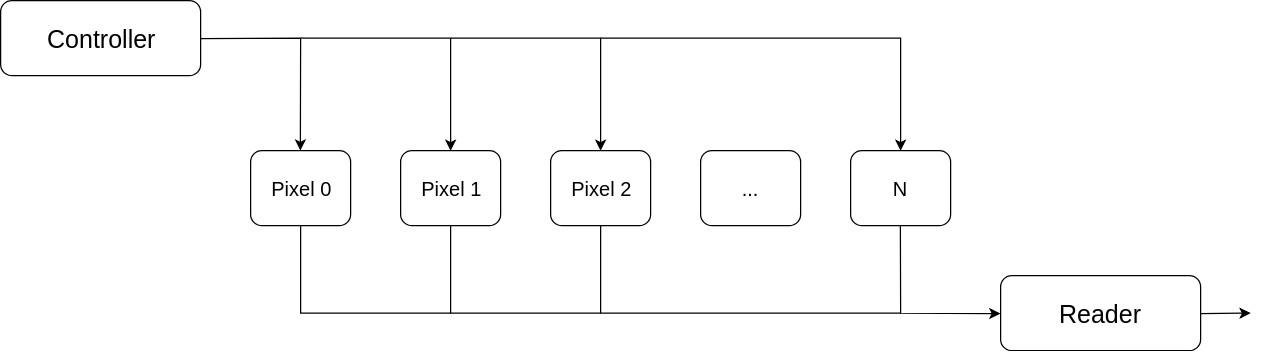
\includegraphics[scale=0.25]{figures/Linedetector.png}
          \caption{The linedetector structure.}
     \end{figure}
\end{frame}

\begin{frame}{Linedetector in \cspm{}}
     \begin{figure}[!ht]
          \centering
          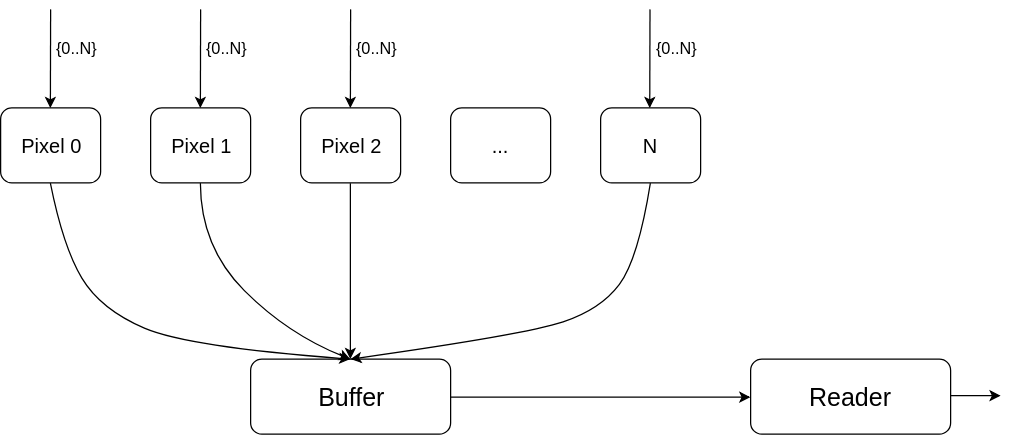
\includegraphics[scale=0.25]{figures/Linedetector_buffer.png}
          \caption{The linedetector structure with buffer.}
     \end{figure}
\end{frame}


\begin{frame}{Linedetector process code}
      \begin{block}{}
       \texttt{\cspm{}} code:
         \vspace{5mm}

          \scalebox{0.8}{\usebox{\cspmlinedetectprocesses}}
      \end{block}
\end{frame}

\begin{frame}{Linedetector buffer code}
      \begin{block}{}
       \texttt{\cspm{}} code:
         \vspace{5mm}

          \scalebox{0.8}{\usebox{\cspmlinedetectbuffer}}
      \end{block}
\end{frame}

\begin{frame}{Linedetector verification}
     Video
\end{frame}

\section{Runtime results}
%%%
%%%%%%%%%%%%%%%%%%%%%%%
%
%%%%%%%%%%%%%%%%%%%%%%%%%%%%%%%%%%
%%% Runtime experiments - seven segments display example
\begin{frame}{Seven segment display clock}
 \begin{block}{}
   \begin{figure}[!ht]
        \tikz{
          \node[inner sep=5pt, outer sep=2pt, draw=blue, fill=black] {
            \sevensegnum[size=1.7em, shrink=0.1]{1}
            \sevensegnum[size=1.7em, shrink=0.1]{2}
          }
        }
        \tikz{
          \node[inner sep=5pt, outer sep=2pt, draw=blue, fill=black] {
            \sevensegnum[size=1.7em, shrink=0.1]{3}
            \sevensegnum[size=1.7em, shrink=0.1]{4}
          }
        }
        \tikz{
          \node[inner sep=5pt, outer sep=2pt, draw=blue, fill=black] {
            \sevensegnum[size=1.7em, shrink=0.1]{5}
            \sevensegnum[size=1.7em, shrink=0.1]{6}
          }
        }
      \setlength{\belowcaptionskip}{-4pt}
      \caption{Digital clock with six seven segment displays, displaying 12:34:56.}
      \label{fig:6_displays}
   \end{figure}
 \end{block}

 \pause

 \begin{block}{}
   Seconds since midnight are calculated into hours, minutes and seconds respectively.
 \end{block}

 \pause

 \begin{block}{}
   One seven segment display can only display the numbers 0-9. \\
   4 bits can represent 0-15, which is more than needed.
 \end{block}

  \pause

  \begin{block}{}
    We can verify that the values communicated does not exceed the expected values.
  \end{block}

\end{frame}




%%%
%%%%%%%%%%%%%%%%%%%%%%%
%
%%%%%%%%%%%%%%%%%%%%%%%%%%%%%%%%%%
%%% Runtime experiments - new results

\begin{frame}{Number of visited states - Clocked and Original}
         \begin{columns}[t, totalwidth=1.02\textwidth]
             \begin{column}{0.50\linewidth}
                 % \begin{block}{}
\begin{figure}[!ht]
     \centering
     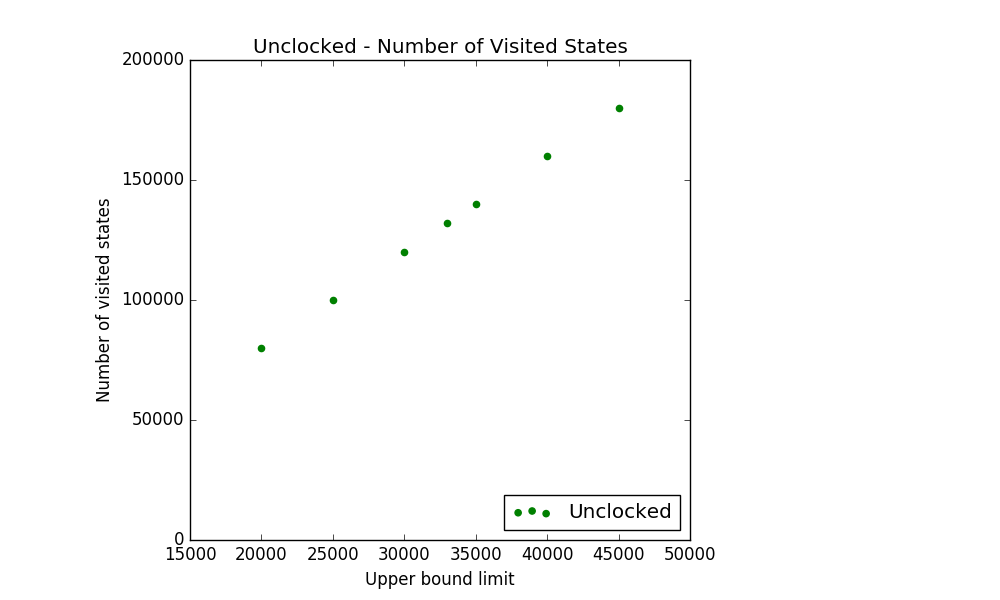
\includegraphics[scale=0.28]{figures/unclocked_states.png}
     \caption{Unclocked number of visited states}
\end{figure}
                 % \end{block}
             \end{column}

             \begin{column}{0.50\linewidth}
                 % \begin{block}{Clocked TAPS}
\begin{figure}[!ht]
     \centering
     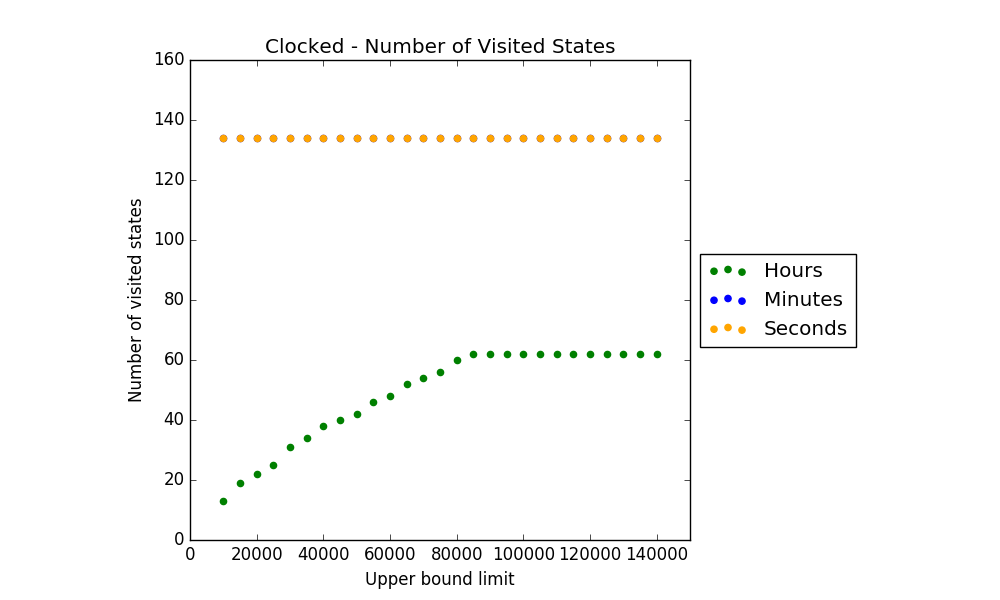
\includegraphics[scale=0.28]{figures/clocked_states.png}
     \caption{Clocked number of visited states}
\end{figure}
                 % \end{block}
             \end{column}

         \end{columns}
\end{frame}

\begin{frame}{Verification time - Clocked and Original}
         \begin{columns}[t, totalwidth=1.02\textwidth]
             \begin{column}{0.50\linewidth}
                 % \begin{block}{}
\begin{figure}[!ht]
     \centering
     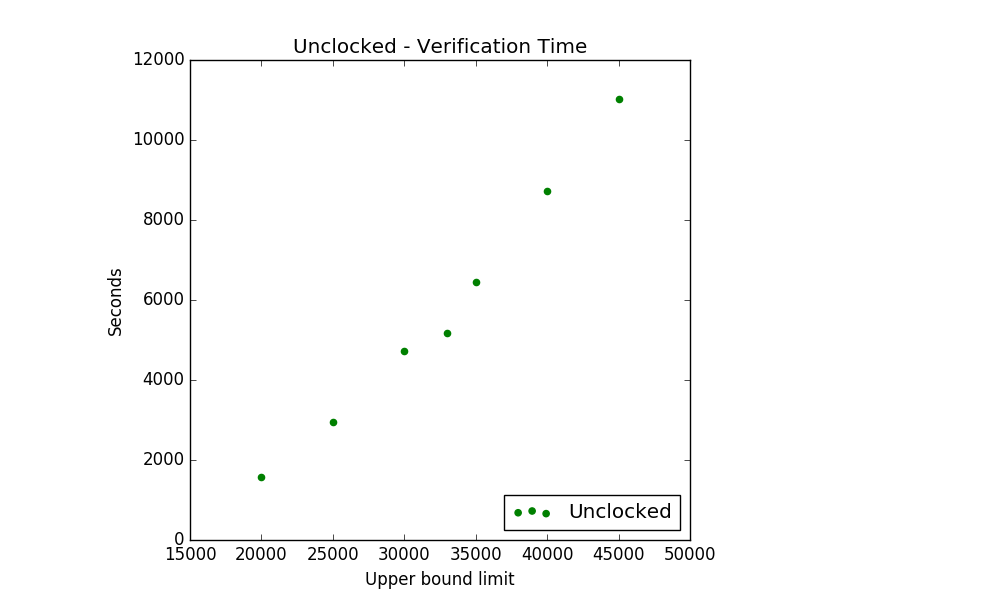
\includegraphics[scale=0.28]{figures/unclocked_verification_time.png}
     \caption{Unclocked verification time}
\end{figure}
                 % \end{block}
             \end{column}

             \begin{column}{0.50\linewidth}
                 % \begin{block}{Clocked TAPS}
\begin{figure}[!ht]
     \centering
     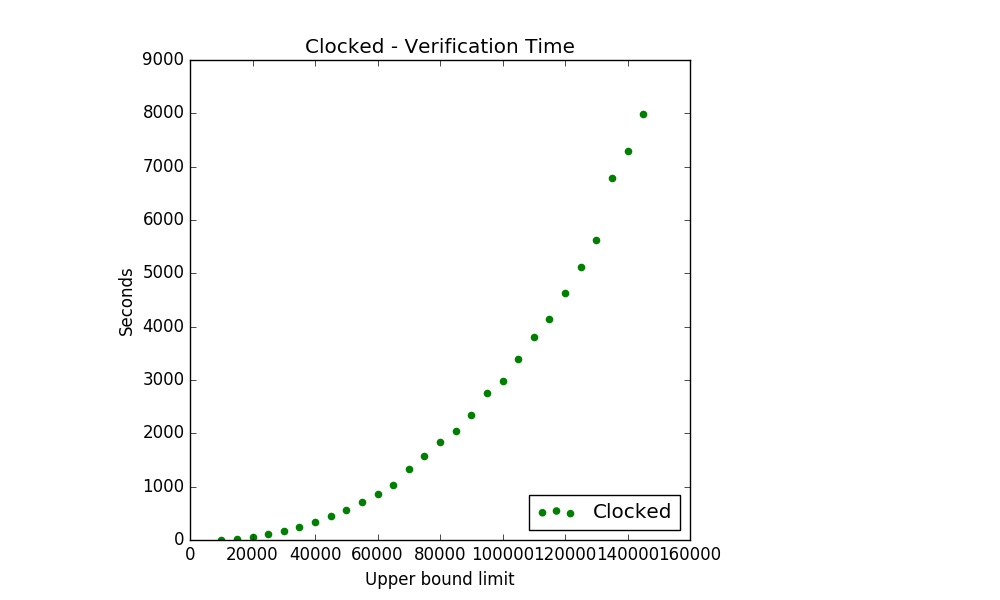
\includegraphics[scale=0.28]{figures/clocked_verification_time.png}
     \caption{Clocked verification time}
\end{figure}
                 % \end{block}
             \end{column}

         \end{columns}
\end{frame}

\begin{frame}{Maximum resident set size - Clocked and Original}
         \begin{columns}[t, totalwidth=1.02\textwidth]
             \begin{column}{0.50\linewidth}
                 % \begin{block}{}
\begin{figure}[!ht]
     \centering
     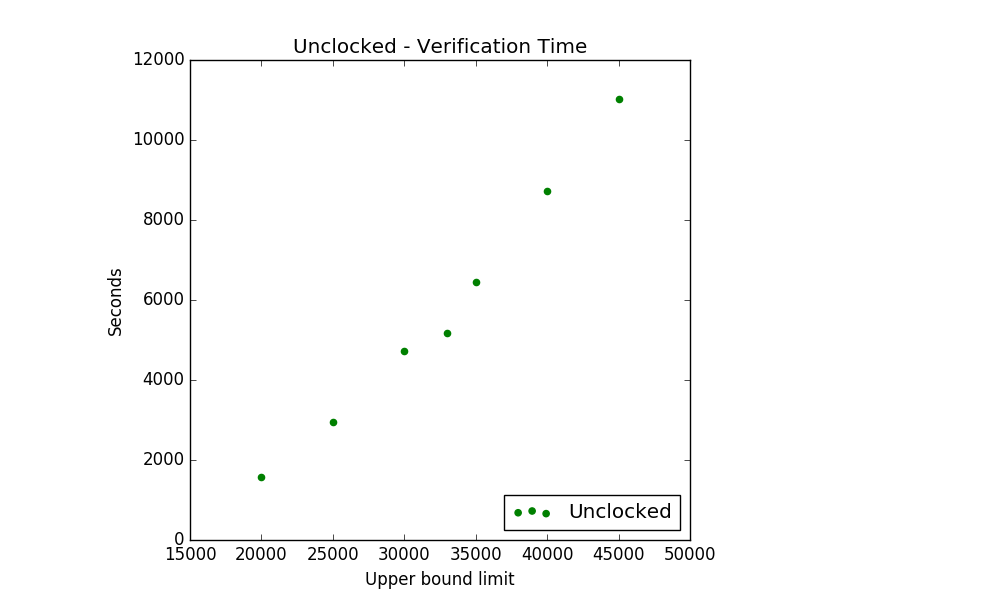
\includegraphics[scale=0.28]{figures/unclocked_verification_time.png}
     \caption{Unclocked maximum resident set size}
\end{figure}
                 % \end{block}
             \end{column}

             \begin{column}{0.50\linewidth}
                 % \begin{block}{Clocked TAPS}
\begin{figure}[!ht]
     \centering
     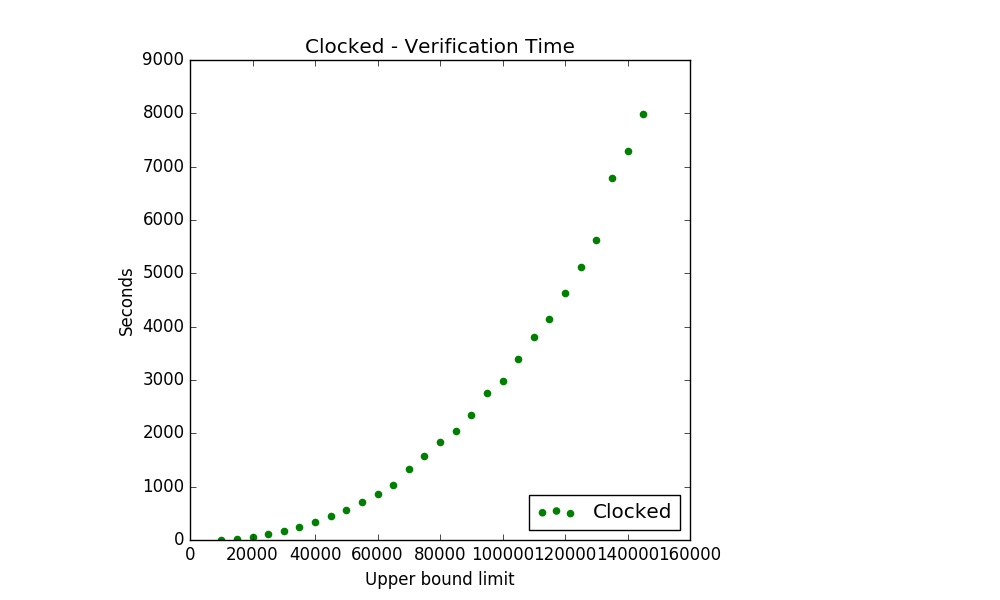
\includegraphics[scale=0.28]{figures/clocked_verification_time.png}
     \caption{Clocked maximum resident set size}
\end{figure}
                 % \end{block}
             \end{column}

         \end{columns}
\end{frame}



\begin{frame}{Increase in processes - Combined}
    \begin{figure}[!ht]
         \centering
         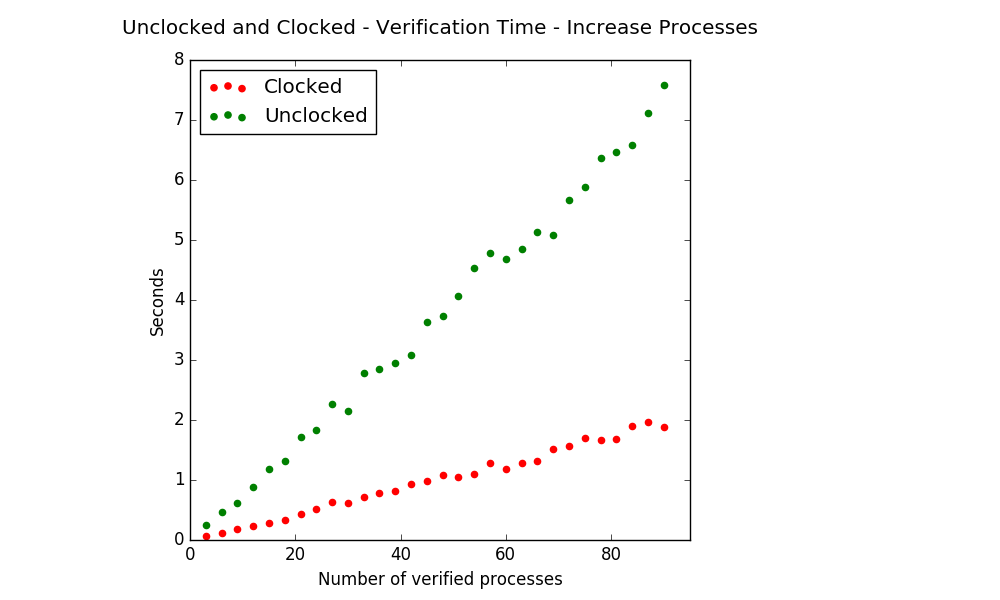
\includegraphics[scale=0.3]{figures/combined_verification_time_increase_proccess.png}
         \caption{Combined verification time}
    \end{figure}

\end{frame}


\begin{frame}{Increase in processes - Combined}
\begin{figure}[!ht]
     \centering
     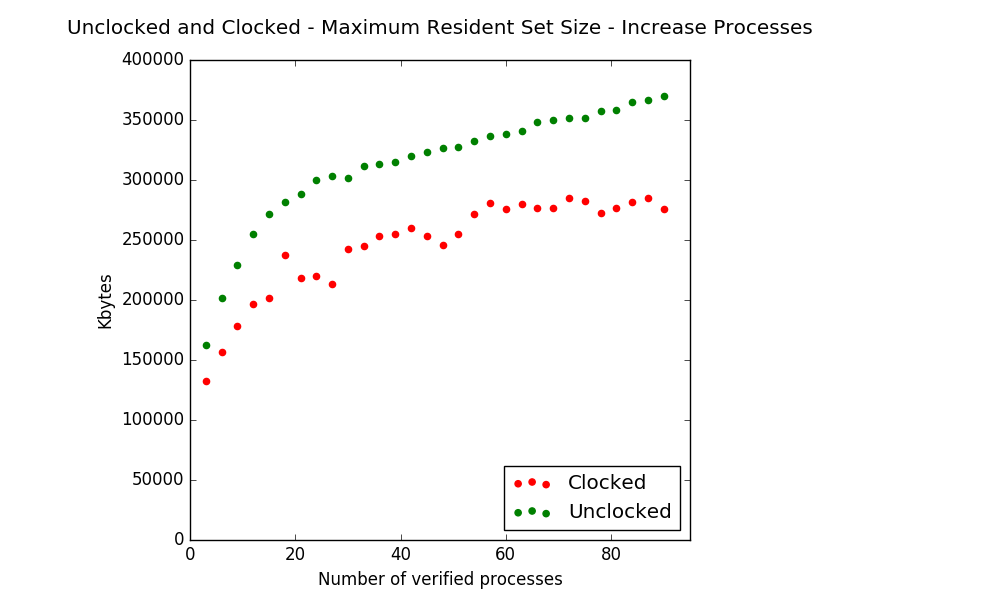
\includegraphics[scale=0.3]{figures/combined_size_time_increase_proccess.png}
     \caption{Combined maximum resident set size}
\end{figure}
\end{frame}

%%%
%%%%%%%%%%%%%%%%%%%%%%%
%
%%%%%%%%%%%%%%%%%%%%%%%%%%%%%%%%%%
%%% Runtime experiments - conclusion
\begin{frame}{How can we use this?}

\begin{block}{}
The original version does not seem to be feasible to use, but the clocked version show great promise.
\end{block}

\pause

\begin{block}{}
More experimentation is needed.
\end{block}

\end{frame}


\section{Future work}
%%%
%%%%%%%%%%%%%%%%%%%%%%%
%
%%%%%%%%%%%%%%%%%%%%%%%%%%%%%%%%%%
%%% Future work
\begin{frame}{Future work}

\begin{block}{}
Advanced assertions.
\end{block}

\pause

\begin{block}{}
Extend for co-simulation.
\end{block}

\pause

\begin{block}{}
Exchange verified elements with equivalent smaller processes might reduce verification time.
\end{block}


\end{frame}

%%%
%%%%%%%%%%%%%%%%%%%%%%%
%
%%%%%%%%%%%%%%%%%%%%%%%%%%%%%%%%%%
%%% The end
  \begin{frame}
  \vfill
  \centering
  \begin{beamercolorbox}[sep=8pt,center,shadow=true,rounded=true]{title}
    \usebeamerfont{title}Thank you!\par%
  \end{beamercolorbox}
  \vfill
  \end{frame}



% %%%%%%%%%%%%%%%%%%%%%%%%%%%%%%%%%%%%%%%%%%%%%%%%%%%%%%%%%%%%%%%%%%%%%%%%
%%%
%%%%%%%%%%%%%%%%%%%%%%%
%
%%%%%%%%%%%%%%%%%%%%%%%%%%%%%%%%%%
%%% What can SME do?
% \begin{frame}{How do we use SME?}
%  \begin{block}{}
%    The SME model builds on the CSP algebra and therefore all SME models have a corresponding CSP model.
%
%  \end{block}
%
%  \pause
%
%   \begin{block}{}
%     We transpile not only the SME network, but also all the SME processes and their content.
%   \end{block}
%
%  \pause
%
%   \begin{block}{}
%     We can translate SME sequentially which simplifies the transpilation.
%   \end{block}
% \end{frame}
%%
%%%%%%%%%%%%%%%%%%%%%%%%%%%%%%%%%%%%
%
%%%%%%%%%%%%%%%%%%%%%%%%%%%
%% SMEIL
% \begin{frame}{How do we use SMEIL?}
%  \begin{block}{}
%     Introduced by Truls Asheim in the previous presentation.
%  \end{block}
%
%  \pause
%
%  \begin{block}{}
%    We transpile from SMEIL to \cspm{}.\\
%    And then verify it in FDR4.
%  \end{block}
%
%  \pause
%
%  \begin{block}{}
%    The transpiler currently only works with pure SMEIL programs.
%  \end{block}
% \end{frame}
%%
%%%%%%%%%%%%%%%%%%%%%%%%%%%%%%%%%%%%
%
%%%%%%%%%%%%%%%%%%%%%%%%%%%
%% Simple example
% \begin{frame}{Seven segment display clock}
%  \begin{block}{}
%    \begin{figure}[!ht]
%         \tikz{
%           \node[inner sep=5pt, outer sep=2pt, draw=blue, fill=black] {
%             \sevensegnum[size=2em, shrink=0.1]{1}
%             \sevensegnum[size=2em, shrink=0.1]{2}
%           }
%         }
%         \tikz{
%           \node[inner sep=5pt, outer sep=2pt, draw=blue, fill=black] {
%             \sevensegnum[size=2em, shrink=0.1]{3}
%             \sevensegnum[size=2em, shrink=0.1]{4}
%           }
%         }
%         \tikz{
%           \node[inner sep=5pt, outer sep=2pt, draw=blue, fill=black] {
%             \sevensegnum[size=2em, shrink=0.1]{5}
%             \sevensegnum[size=2em, shrink=0.1]{6}
%           }
%         }
%       \caption{Digital clock with six seven segment displays, displaying 12:34:56.}
%       \label{fig:6_displays}
%    \end{figure}
%  \end{block}
%
%  \pause
%
%  \begin{block}{}
%    Seconds since midnight.
%  \end{block}
%
%  \pause
%
%  \begin{block}{}
%    Arithmetics calculate hours, minutes and seconds respectively.
%  \end{block}
%
%  \pause
%
%  \begin{block}{}
%   Two seven segment displays pr. \texttt{time} process.
%  \end{block}
%
% \end{frame}
%
%
% \begin{frame}{Seven segment display clock}
%  \begin{block}{}
%   \begin{figure}[!ht]
%   \centering
%   \begin{tikzpicture}
%     \node [mycircle] (I) at (0,0) {$I$};
%
%     \node [mycircle] (H) at (2.5,  1.50) {$H$};
%     \node [mycircle] (M) at (2.5,  0.00) {$M$};
%     \node [mycircle] (S) at (2.5, -1.50) {$S$};
%
%     \draw [myarrow] (I) -- (M);
%
%     \draw [myarrow, smooth] (I) to[out=0, in=180] (H);
%     \draw [myarrow, smooth] (I) to[out=0, in=180] (S);
%
%     % Output arrows without processes
%     \draw [myarrow] (3.125,  1.625) -- (4.000,  1.750);
%     \draw [myarrow] (3.125,  1.375) -- (4.000,  1.250);
%     \draw [myarrow] (3.125,  0.125) -- (4.000,  0.250);
%     \draw [myarrow] (3.125, -0.125) -- (4.000, -0.250);
%     \draw [myarrow] (3.125, -1.375) -- (4.000, -1.250);
%     \draw [myarrow] (3.125, -1.625) -- (4.000, -1.750);
%   \end{tikzpicture}
%   \caption{SMEIL network for a seven segment display clock. Each SMEIL process is represented by a cicle with a letter corresponding to the processes Input, Hours, Minutes and Seconds respectively.}
%   \label{fig:smeil_network}
% \end{figure}
%  \end{block}
% \end{frame}
%
% \begin{frame}{What are we verifying?}
%  \begin{block}{}
%    One seven segment display can only display the numbers 0-9. \\
%    4 bits can represent 0-15, which is more than needed.
%  \end{block}
%
%  \pause
%
%  \begin{block}{}
%    We can verify that the values communicated to all the seven segment displays does not exceed the expected values.
%  \end{block}
%
%   \pause
%
%   \begin{block}{}
%     In this case we can restrict the assertions further. \\
%     The time will never be more than 23:59:59.
%   \end{block}
%
%
%  \pause
%
%  \begin{block}{}
%    In general, we verify the values comnmunicated on \cspm{} channels.
%  \end{block}
% \end{frame}
%
% \begin{frame}{Seven Segment display clock}
%  \begin{block}{}
%   \texttt{SMEIL} code:
%     \vspace{5mm}
%
%      \scalebox{0.8}{\usebox{\smeilexamplecode}}
%  \end{block}
% \end{frame}
%%
%%%%%%%%%%%%%%%%%%%%%%%%%%%%
%
%%%%%%%%%%%%%%%%%%%%%%%%%%%%%%
%% Now for the transpiling
% \begin{frame}{The transpiling}
%  \begin{block}{}
%    SMEIL bus to \cspm{} channel.
%  \end{block}
%
%  \pause
%
%  \begin{block}{}
%    \cspm{} process structure.
%  \end{block}
%
%  \pause
%
%  \begin{block}{}
%    The monitor process.
%  \end{block}
% \end{frame}

%%
%%%%%%%%%%%%%%%%%%%%%%%%%%%%
%
%%%%%%%%%%%%%%%%%%%%%%%%%%%%%%
%% SMEIL bus to \cspm{} channel
% \begin{frame}{SMEIL bus to \cspm{} channel}
%  \begin{block}{}
%    \texttt{SMEIL} code:
%      \vspace{5mm}
%
%       \scalebox{0.8}{\usebox{\smeilchannelexample}}
%  \end{block}
%  \pause
%  \begin{block}{}
%     \texttt{\cspm{}} code:
%       \vspace{5mm}
%
%        \scalebox{0.8}{\usebox{\cspmchannelexample}}
%  \end{block}
% \end{frame}

%%
%%%%%%%%%%%%%%%%%%%%%%%%%%%%
%
%%%%%%%%%%%%%%%%%%%%%%%%%%%%%%
%% \cspm{} process structure
% \begin{frame}{\cspm{} process structure}
%  \begin{block}{}
%    \texttt{SMEIL} code:
%      \vspace{5mm}
%
%       \scalebox{0.8}{\usebox{\smeilprocessexample}}
%  \end{block}
%  \pause
%  \begin{block}{}
%     \texttt{\cspm{}} code:
%       \vspace{5mm}
%
%        \scalebox{0.8}{\usebox{\cspmprocessexample}}
%  \end{block}
%
% \end{frame}
%%
%%%%%%%%%%%%%%%%%%%%%%%%%%%%%%%
%
%%%%%%%%%%%%%%%%%%%%%%%%%%%%
%% Monitor process
% \begin{frame}{The monitor process}
%  \begin{block}{}
%      \begin{figure}[!ht]
%       \centering
%       \begin{tikzpicture}[auto]
%         \node[mycircle] (P) at (-1.5, 0.0) {$P$};
%         \node[mycircle] (Q) at ( 2.5, 0.0) {$Q$};
%         \node[mycircle, shape=rectangle] (M) at ( 0.5, 1.5) {$M$};
%
%         \node[draw, shape=circle, inner sep=0pt, minimum size=5pt] (m) at (0.5, 0.0) {};
%
%
%         \draw (M) -- (P -| M) [black!50];
%         \draw [myarrow] (P) -- (Q);
%       \end{tikzpicture}
%       \caption{The monitor process \textit{M} listens in on the communication between \textit{P} and \textit{Q} in order to assert the communicated values.}
%       \label{fig:assertion_process}
%     \end{figure}
%  \end{block}
% \end{frame}
% \begin{frame}{The monitor process}
%  \begin{block}{}
%    \texttt{SMEIL} code:
%      \vspace{5mm}
%
%       \scalebox{0.8}{\usebox{\smeilchannelexample}}
%  \end{block}
%  \pause
%  \begin{block}{}
%     \texttt{\cspm{}} code:
%       \vspace{5mm}
%
%        \scalebox{0.8}{\usebox{\cspmmonitorexample}}
%  \end{block}
%
% \end{frame}
%%
%%%%%%%%%%%%%%%%%%%%%%%%%%%%%
%
%%%%%%%%%%%%%%%%%%%%%%%
%% Example continued
% \begin{frame}{Seven segment display clock}
%  \begin{block}{}
%   \texttt{\cspm{}} code:
%     \vspace{3mm}
%
%      \scalebox{0.7}{\usebox{\cspmexample}}
%  \end{block}
% \end{frame}
%%
%%%%%%%%%%%%%%%%%%%%%%%%%%%%%
%
%%%%%%%%%%%%%%%%%%%%%%%
%% Example continued
% \begin{frame}{Seven segment display clock}
%      \begin{figure}[!ht]
%           \centering
%           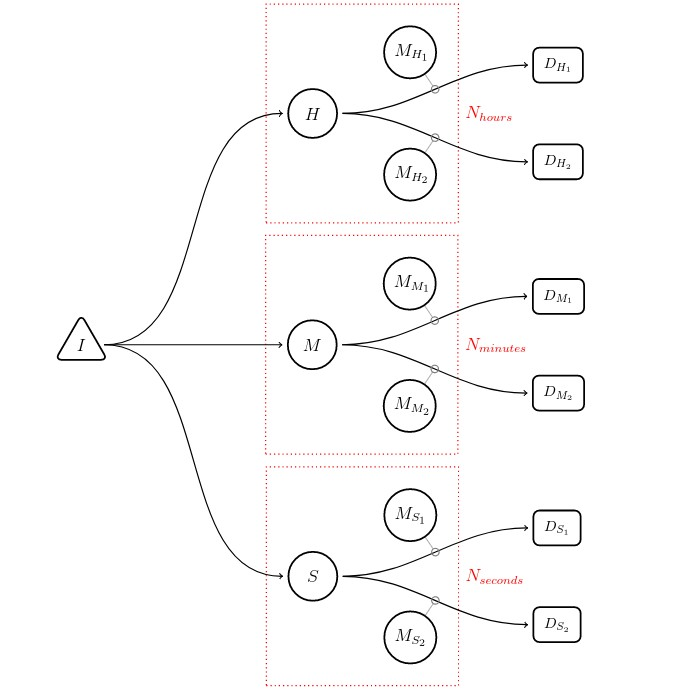
\includegraphics[scale=0.295]{cspm_figure.jpg}
%           \caption{A seven segment display clock network in \cspm{}.}
%           \label{fig:cspm-network}
%      \end{figure}
% \end{frame}

%%
%%%%%%%%%%%%%%%%%%%%%%%%%%%%%
%
%%%%%%%%%%%%%%%%%%%%%%%
%% Results - time to verify in FDR4?
% \begin{frame}{Verification in FDR4}
%  \begin{block}{}
%      The seven segment example have been run on a Intel(R) Xeon(R) CPU E5-2698 v4 @ 2.20GHz.
%
%      \vspace{5mm}
%      We had a few problems with FDR4, but dividing the task was possible in this case.
%
%      \vspace{5mm}
%      When dividing the task, 0 to 131071 seconds can be verified in $\approx$ 2 hours 40 minutes.
%  \end{block}
% \end{frame}
%%
%%%%%%%%%%%%%%%%%%%%%%%%
%
%%%%%%%%%%%%%
%% Conclusion
% \begin{frame}{Conclusion}
%  \begin{block}{}
%   With this system we can transpile hardware models to \cspm{}.
%  \end{block}
%
%  \pause
%
%  \begin{block}{}
%   Verify values on the \cspm{} channels.
%  \end{block}
%
%  \pause
%
%  \begin{block}{}
%   Verify the original hardware model.
%  \end{block}
%
%  \pause
%
%  \begin{block}{}
%   Extract specification.
%  \end{block}
%
% \end{frame}
%% /Conclusion
%%%%%%%%%%%%%%
%
%%%%%%%%%%%%%%
%% Future work
% \begin{frame}{Future work}
%  \begin{block}{}
%      Hardware/software co-simulation.
%  \end{block}
%
%  \pause
%
%  \begin{block}{}
%      Creating more extensive examples to show the possibilities of the system.
%  \end{block}
%
% \end{frame}
%% /Future work
%%%%%%%%%%%%%%%
%
%%%%%%%%%%%%%%%
%%%% Questions?
% \begin{frame}{Questions?}
% 	\begin{block}{}
%         Thank you!
% 	\end{block}
% 	% \begin{block}{}
% 	% 	Contact:
%     %     tpq587@alumni.ku.dk
%     %     alberte@thegler.dk
% 	% \end{block}
% \end{frame}
%%%% /Questions?
%%%%%%%%%%%%%%%%

\end{document}
